\pagebreak
\subsubsection{T-SNE}

Se aplicó el algoritmo TSNE descrito en la sección \ref{sec:tsne} con los valores de perplejidad de 100, 200, 300 y 400 con los datos de los años 2015 y 2020. En la figura \ref{fig:tsne_2d} se observan los resultados obtenidos para el caso bidimensional.

\begin{figure}[H]
	\centering
	\begin{subfigure}{8.4cm}
		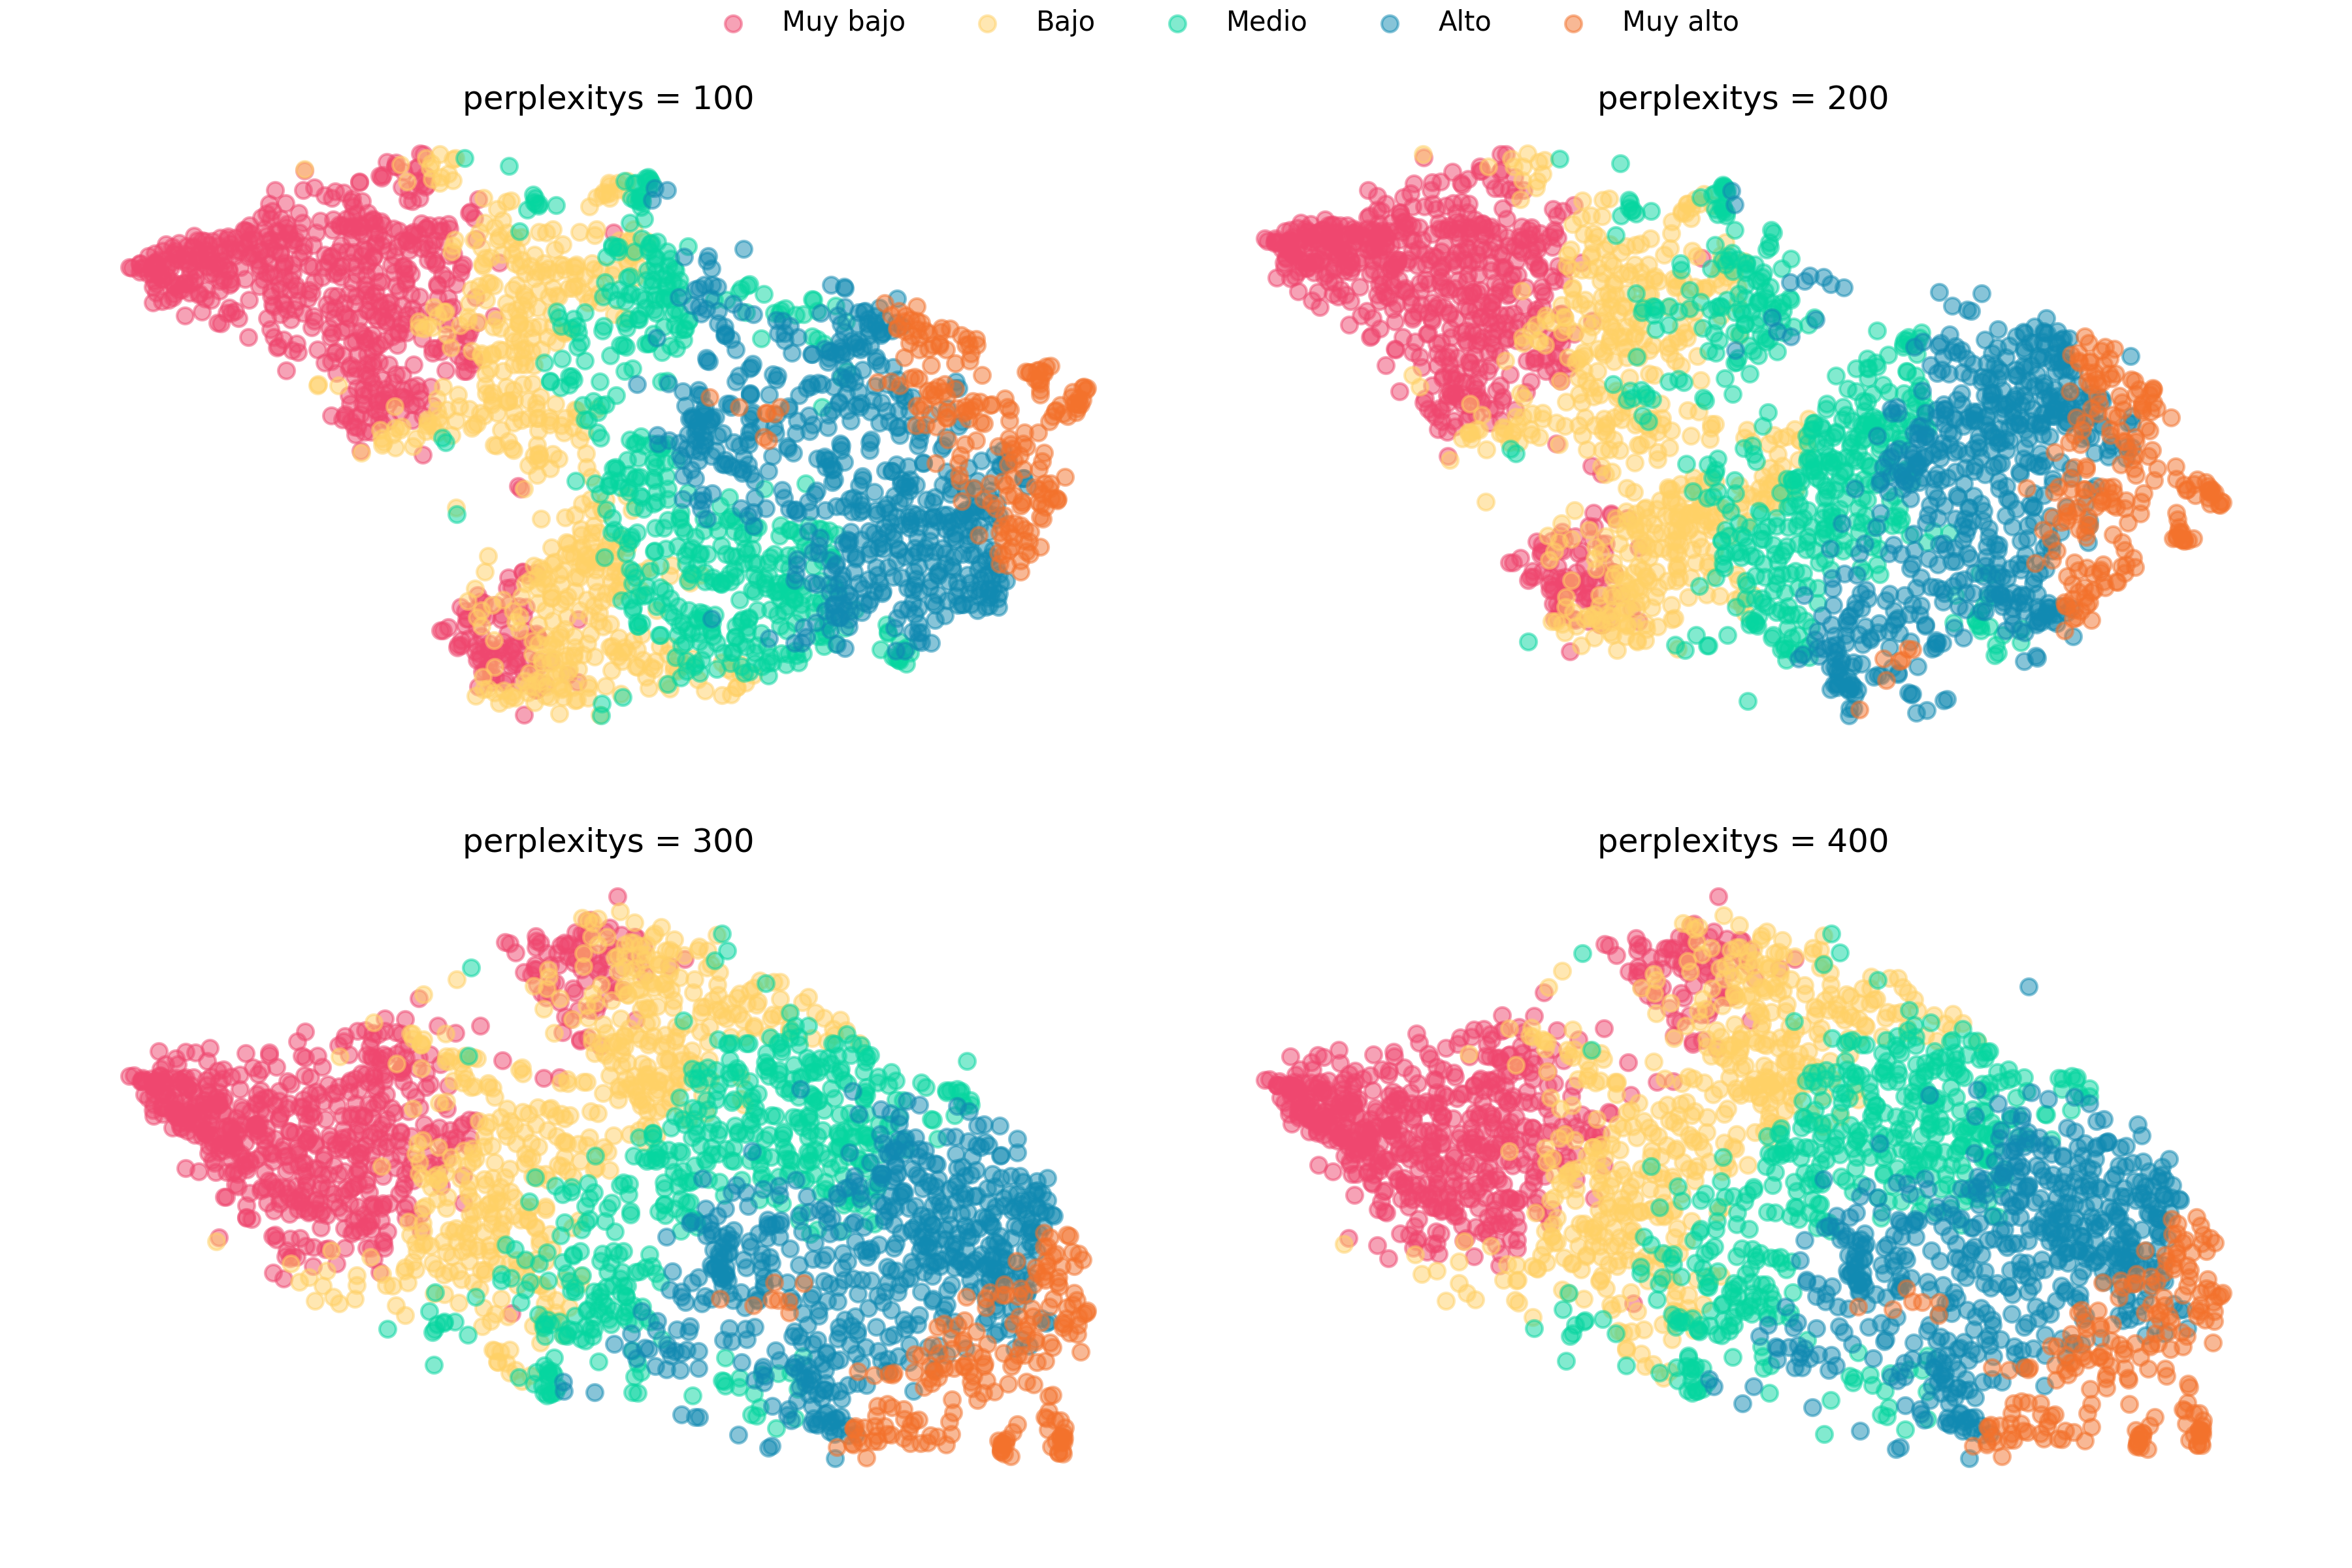
\includegraphics[width=1\linewidth]{Graphics/Data_2015/TSNE_2D.png}
		\caption{Datos 2015}
	\end{subfigure}
	\begin{subfigure}{8.4cm}
		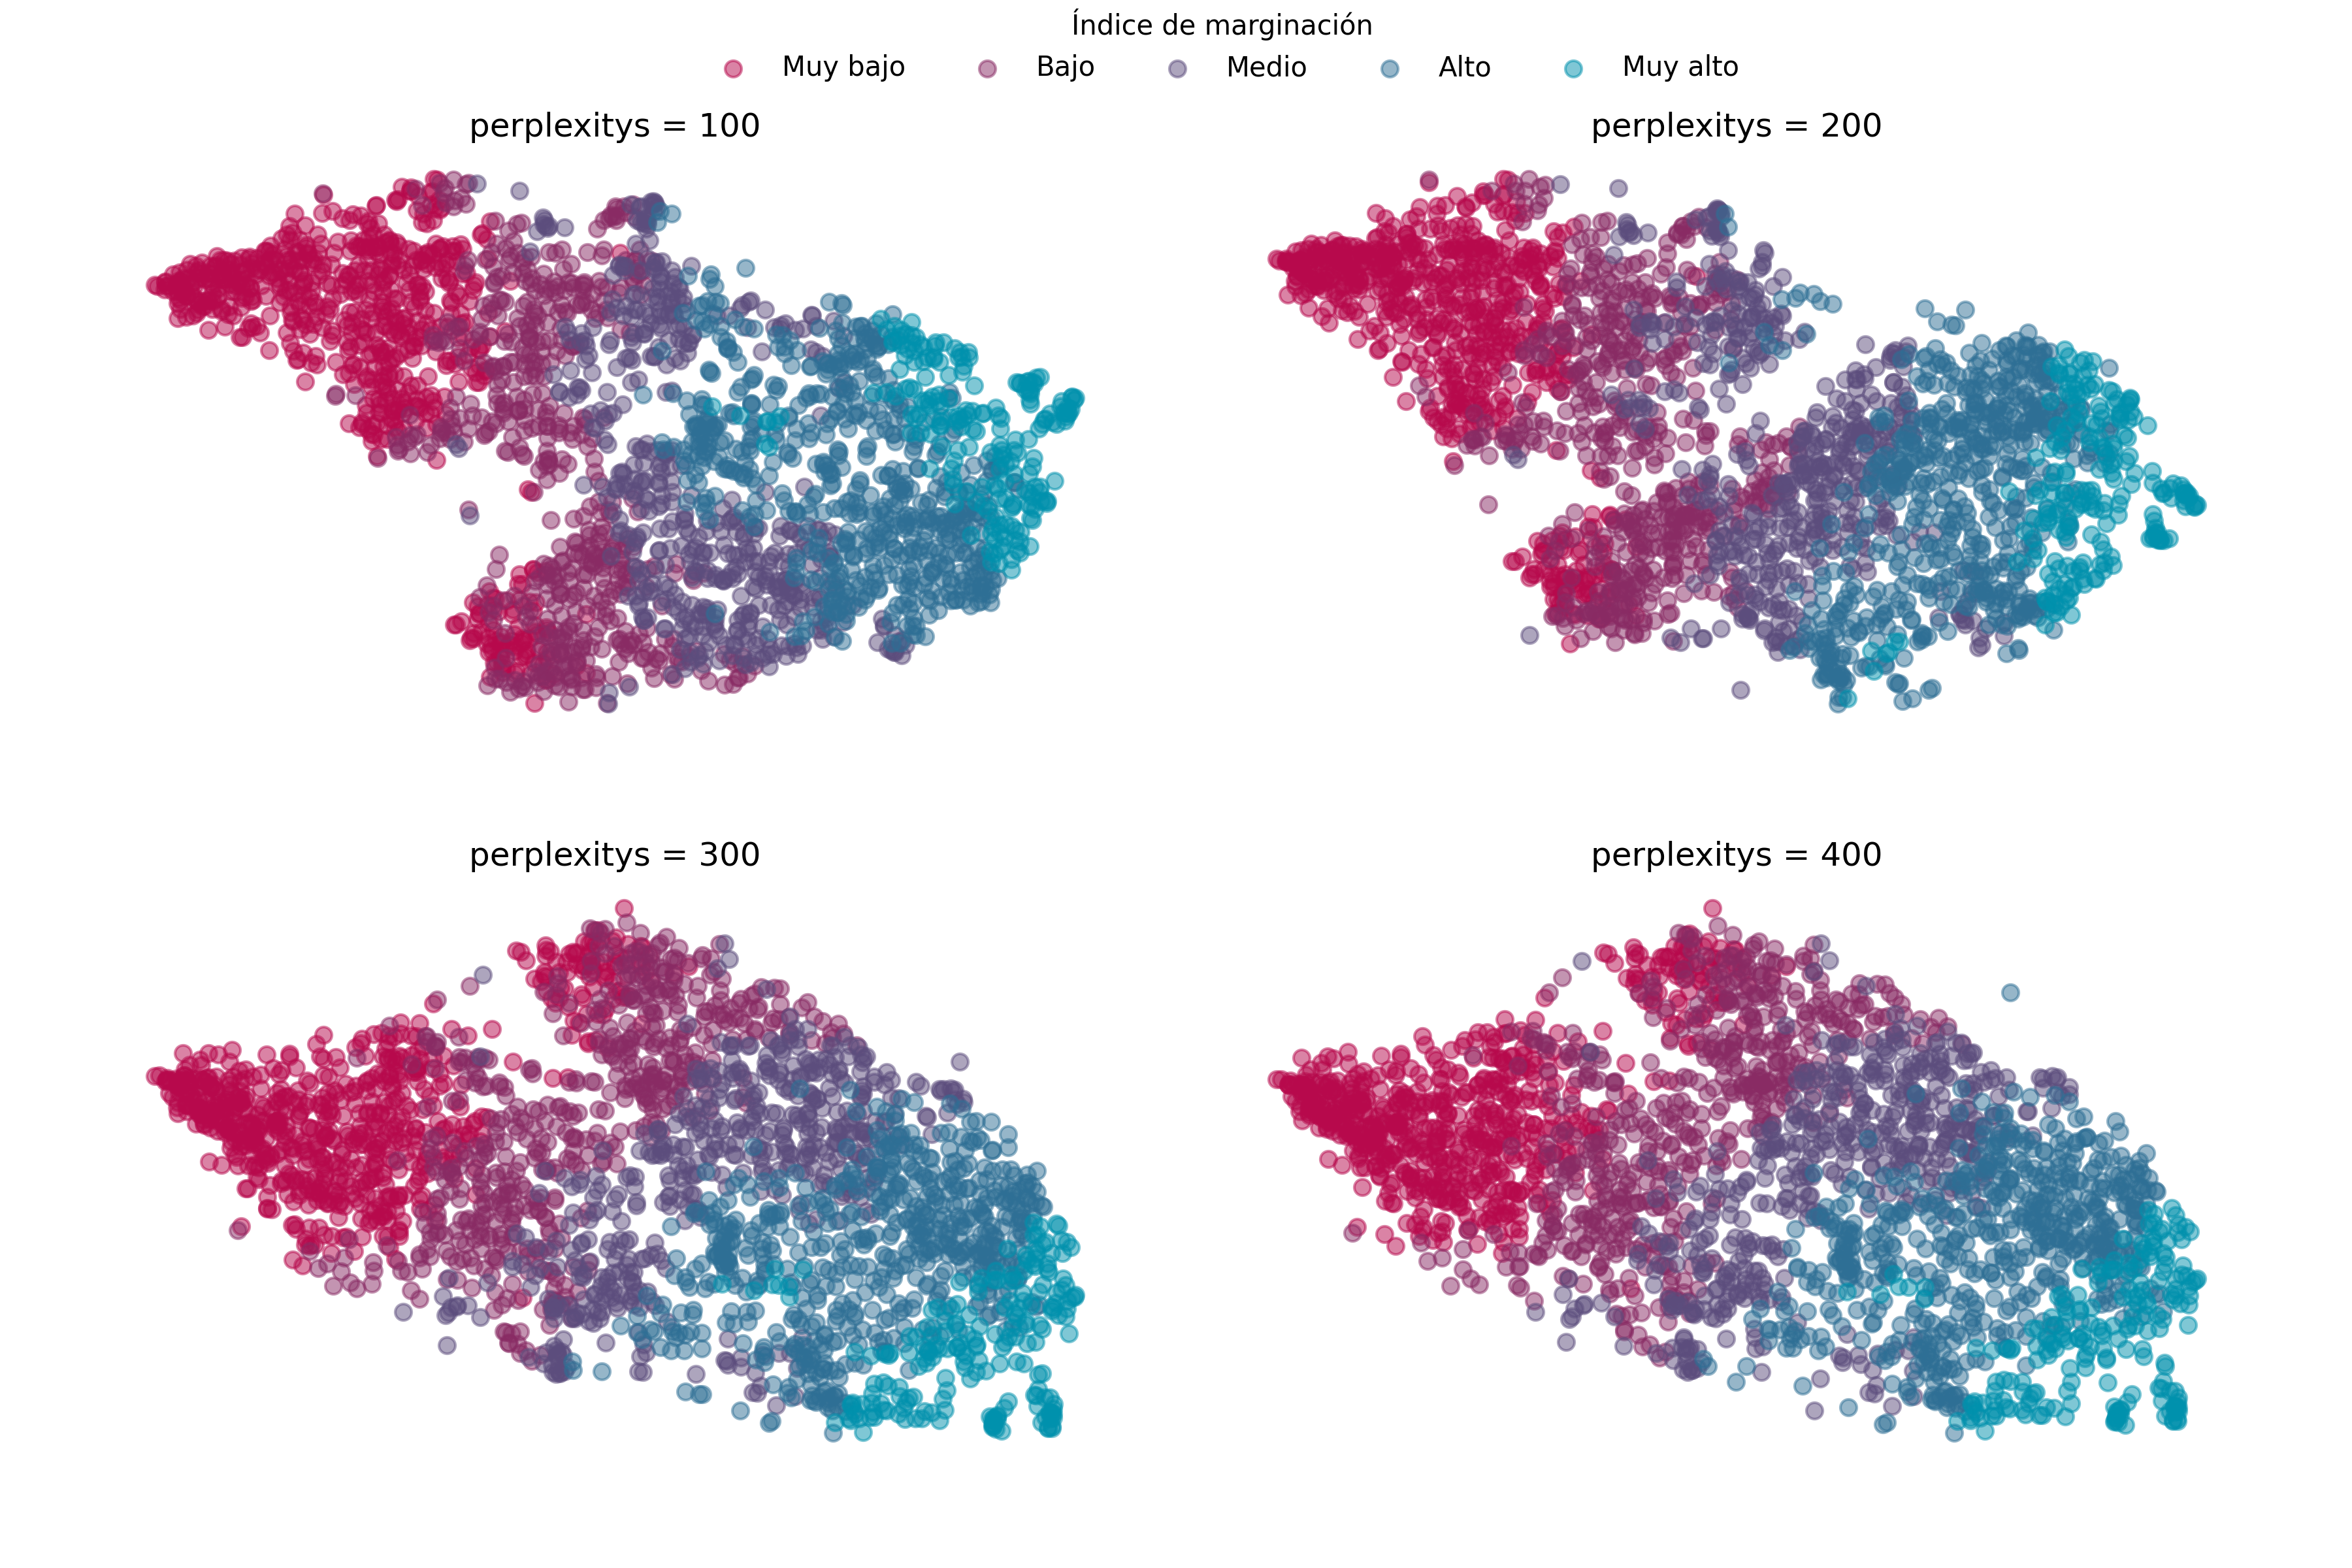
\includegraphics[width=1\linewidth]{Graphics/Data_2020/TSNE_2D.png}
		\caption{Datos 2020}
	\end{subfigure}
	\caption{Resultados de aplicar T-SNE para el caso bidimensional para los datos de índice de marginación de los años 2015 y 2020.}
	\label{fig:tsne_2d}
\end{figure}

En la tabla \ref{table:tsne_results} se pueden descargar las visualizaciones tridimensionales de los resultados del algoritmo ISOMAP en el caso tridimensional.

\begin{table}[H]
	\centering
	\begin{tabular}{lrr} \hline
		\multirow{2}{*}{Perplejidad} & \multicolumn{2}{c}{Años}                                                                                                                                                                                                                                              \\ \cline{2-3}
		                             & 2015                                                                                                                              & 2020                                                                                                                              \\ \hline
		100                          & \href{https://github.com/giovannilopez9808/Reconocimiento_de_patrones_proyecto/raw/main/Graphics/Data_2015/TSNE_3D_100.mp4}{Link} & \href{https://github.com/giovannilopez9808/Reconocimiento_de_patrones_proyecto/raw/main/Graphics/Data_2020/TSNE_3D_100.mp4}{Link} \\
		200                          & \href{https://github.com/giovannilopez9808/Reconocimiento_de_patrones_proyecto/raw/main/Graphics/Data_2015/TSNE_3D_200.mp4}{Link} & \href{https://github.com/giovannilopez9808/Reconocimiento_de_patrones_proyecto/raw/main/Graphics/Data_2020/TSNE_3D_200.mp4}{Link} \\
		300                          & \href{https://github.com/giovannilopez9808/Reconocimiento_de_patrones_proyecto/raw/main/Graphics/Data_2015/TSNE_3D_300.mp4}{Link} & \href{https://github.com/giovannilopez9808/Reconocimiento_de_patrones_proyecto/raw/main/Graphics/Data_2020/TSNE_3D_300.mp4}{Link} \\
		400                          & \href{https://github.com/giovannilopez9808/Reconocimiento_de_patrones_proyecto/raw/main/Graphics/Data_2015/TSNE_3D_400.mp4}{Link} & \href{https://github.com/giovannilopez9808/Reconocimiento_de_patrones_proyecto/raw/main/Graphics/Data_2020/TSNE_3D_400.mp4}{Link} \\ \hline
	\end{tabular}
	\caption{Link de descarga para las visualizaciones tridimensionales de los resultados de T-SNE para 100, 200, 300 y 400 DE perplejidad en los años 2015 y 2020.}
	\label{table:tsne_results}
\end{table}
